% !TeX root = ../main.tex

\chapter{基于图神经网络的计算图耗时预测方法}

\section{图数据结构与特征编码}

\subsection{数据集说明}

本文所使用的数据集是某深度学习编译器(下称 Y 编译器)编译 ResNet-50 \cite{resnet} 模型生成的 MLIR 文件在不同硬件配置下的实际运行时间。

其中,计算图的结构信息由 MLIR \cite{mlir} 给出。MLIR 与计算图的对应关系的示例如图 \ref{fig:graph5} 和图 \ref{fig:graph6} 所示。

\begin{figure}[h]
    \centering
    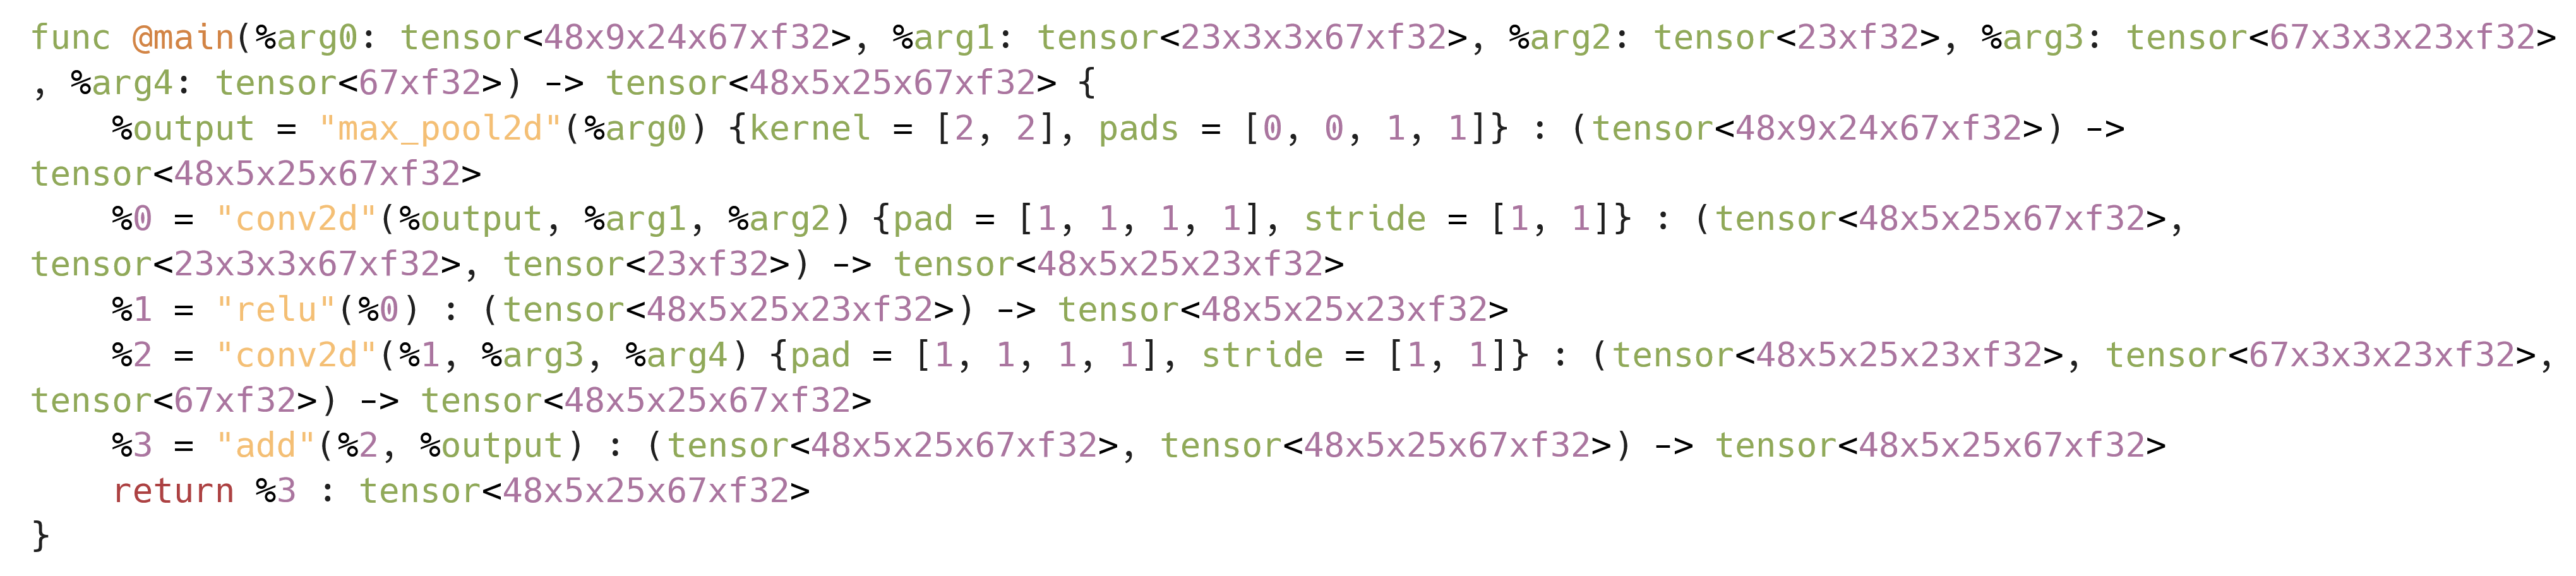
\includegraphics[width=1\textwidth]{figures/mlir.png}
    \caption{MLIR 示例 \cite{mlir_example}}
    \label{fig:graph5}
\end{figure}

\begin{figure}[h]
    \centering
    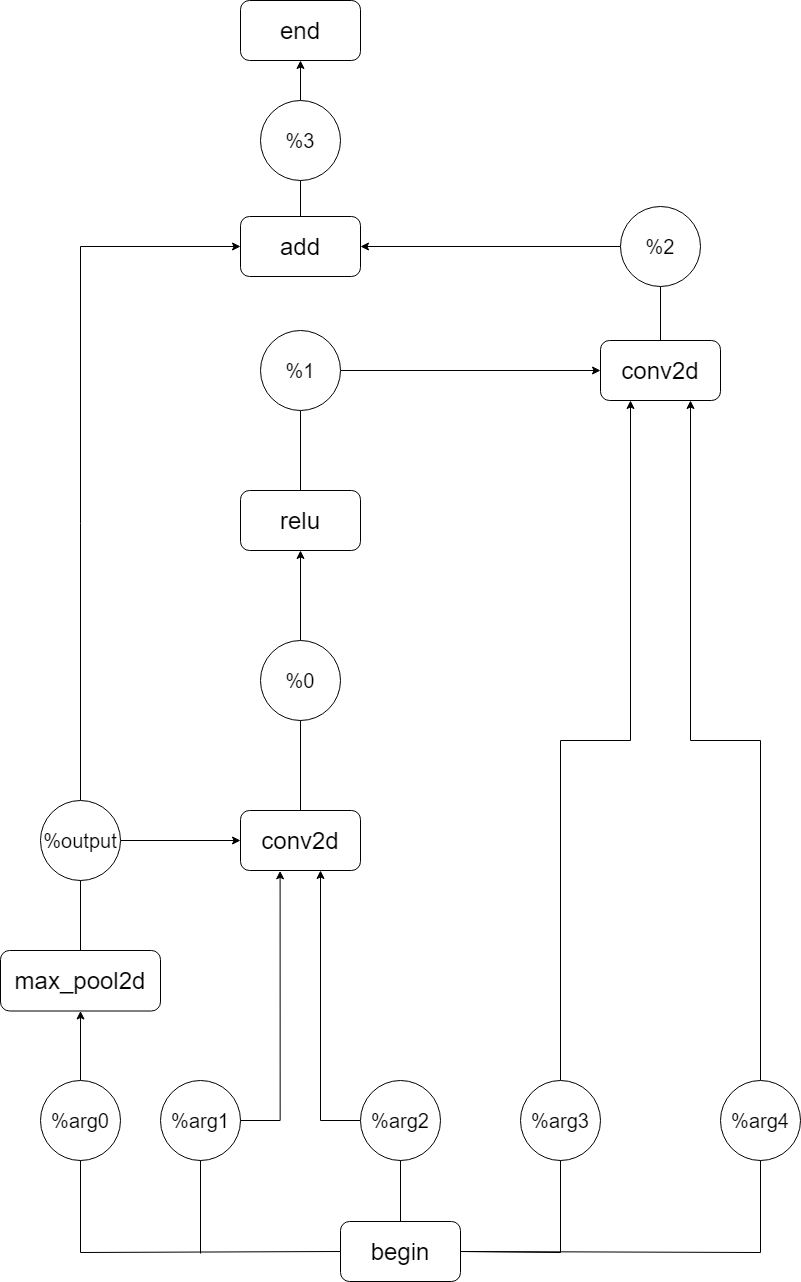
\includegraphics[width=0.5\textwidth]{figures/mlir_cg.png}
    \caption{MLIR 示例对应的计算图}
    \label{fig:graph6}
\end{figure}

如图 \ref{fig:graph7} 所示,硬件配置信息以 Protobuf(.pb)\cite{enwiki:1061454458} 文件的形式给出:

\begin{figure}[h]
    \centering
    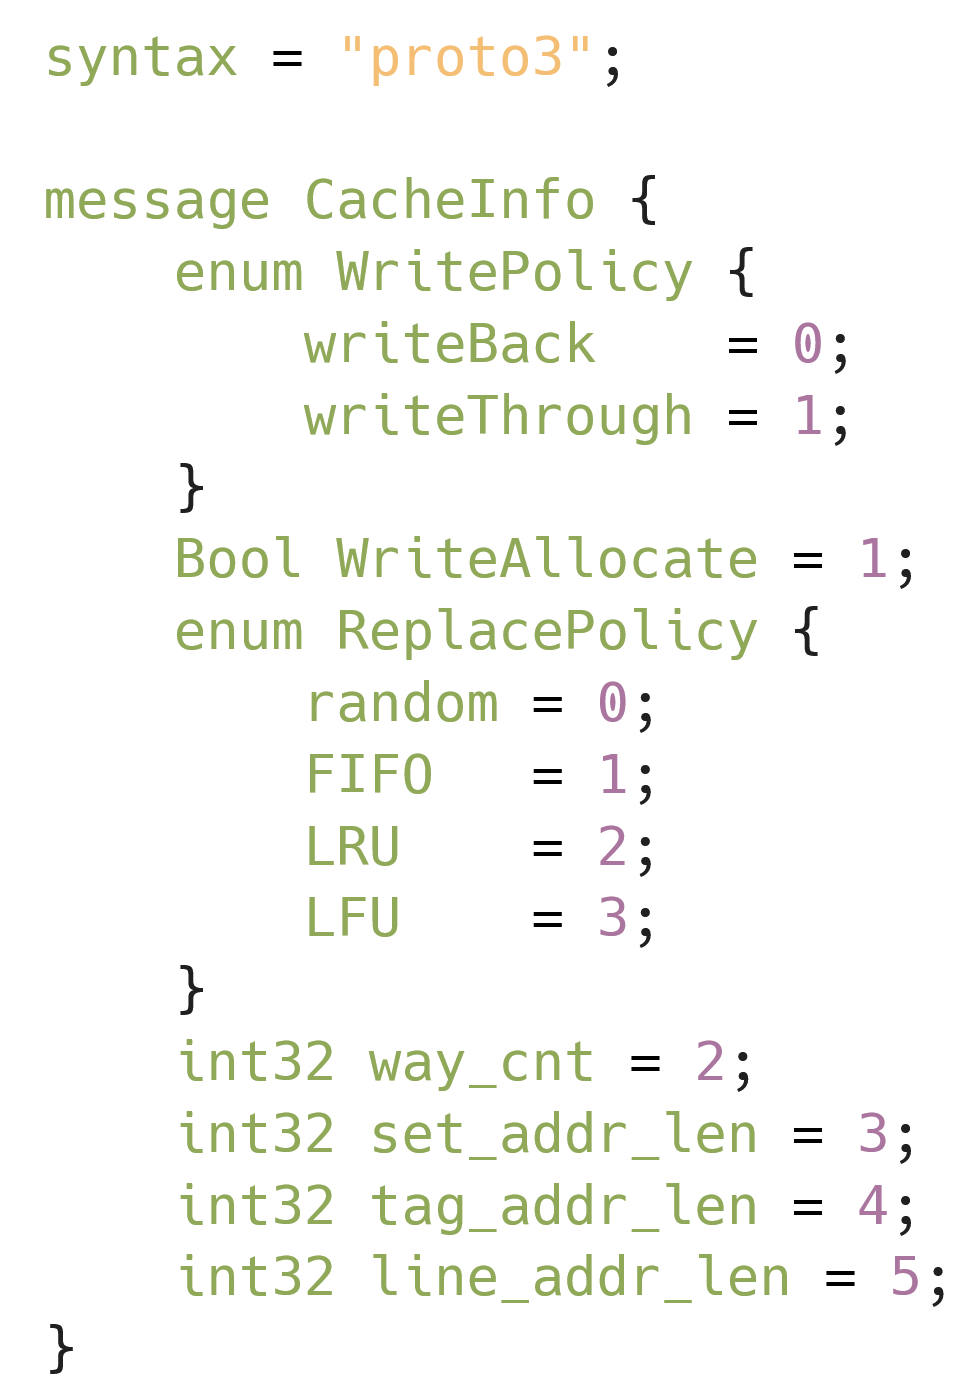
\includegraphics[width=0.3\textwidth]{figures/pb.png}
    \caption{硬件配置示例}
    \label{fig:graph7}
\end{figure}

\subsection{特征编码}
本文所处理的数据特征主要以下三类:

1. 结点的算子特征,如算子的种类,卷积填充的元素个数和步长。

2. 边的张量特征,如张量各个维度的大小和张量的精度类型。

3. 硬件配置特征,如缓存的大小,向量寄存器的个数。这些特征被同一子图的多个结点共享。

此外,对于枚举类型的特征,如算子的数据布局,张量的精度类型以及缓存的替换策略等,由于难以获得种类之间是否相似的先验知识,
本文将它们编码为相互正交的独热码。

表 \ref{tab:table1} 为针对图 \ref{fig:graph6} 的结点自下而上进行特征编码的示例  \footnote{由于篇幅有限,本文对数据集的部分信息进行了简化和模糊处理。本节对数据集和编码方案的介绍仅作为示例,实际数据远比本节的示例复杂。}:

\begin{table}[]
        \centering
        \caption{结点编码示例}
        \begin{threeparttable}
            \scalebox{0.6}{
            \begin{tabular}{|cccccccccccc|}
            \hline
            \multicolumn{1}{|c|}{结点/编码}       & \multicolumn{1}{c|}{结点类型} & \multicolumn{1}{c|}{核大小} & \multicolumn{1}{c|}{填充大小} & \multicolumn{1}{c|}{步长} & \multicolumn{1}{c|}{写回策略}                & \multicolumn{1}{c|}{写分配策略}               & \multicolumn{1}{c|}{替换策略}                  & \multicolumn{1}{c|}{组相联度}               & \multicolumn{1}{c|}{组地址长度}              & \multicolumn{1}{c|}{标签地址长度}             & 行地址长度              \\ \hline
            \multicolumn{1}{|c|}{begin\tnote{a}}        & \multicolumn{1}{c|}{0000} & \multicolumn{1}{c|}{00}  & \multicolumn{1}{c|}{0000} & \multicolumn{1}{c|}{00} & \multicolumn{1}{c|}{00}                  & \multicolumn{1}{c|}{00}                  & \multicolumn{1}{c|}{0000}                  & \multicolumn{1}{c|}{0}                  & \multicolumn{1}{c|}{0}                  & \multicolumn{1}{c|}{0}                  & 0                  \\ \hline
            \multicolumn{1}{|c|}{max\_pool2d}           & \multicolumn{1}{c|}{1000} & \multicolumn{1}{c|}{22\tnote{b}}  & \multicolumn{1}{c|}{0011} & \multicolumn{1}{c|}{00\tnote{c}} & \multicolumn{1}{c|}{\multirow{5}{*}{10\tnote{d}}} & \multicolumn{1}{c|}{\multirow{5}{*}{10}} & \multicolumn{1}{c|}{\multirow{5}{*}{0010}} & \multicolumn{1}{c|}{\multirow{5}{*}{4}} & \multicolumn{1}{c|}{\multirow{5}{*}{3}} & \multicolumn{1}{c|}{\multirow{5}{*}{5}} & \multirow{5}{*}{3} \\ \cline{1-5}
            \multicolumn{1}{|c|}{conv2d}                & \multicolumn{1}{c|}{0100} & \multicolumn{1}{c|}{00}  & \multicolumn{1}{c|}{1111} & \multicolumn{1}{c|}{11} & \multicolumn{1}{c|}{}                    & \multicolumn{1}{c|}{}                    & \multicolumn{1}{c|}{}                      & \multicolumn{1}{c|}{}                   & \multicolumn{1}{c|}{}                   & \multicolumn{1}{c|}{}                   &                    \\ \cline{1-5}
            \multicolumn{1}{|c|}{relu}                  & \multicolumn{1}{c|}{0010} & \multicolumn{1}{c|}{00}  & \multicolumn{1}{c|}{0000} & \multicolumn{1}{c|}{00} & \multicolumn{1}{c|}{}                    & \multicolumn{1}{c|}{}                    & \multicolumn{1}{c|}{}                      & \multicolumn{1}{c|}{}                   & \multicolumn{1}{c|}{}                   & \multicolumn{1}{c|}{}                   &                    \\ \cline{1-5}
            \multicolumn{1}{|c|}{conv2d}                & \multicolumn{1}{c|}{0100} & \multicolumn{1}{c|}{00}  & \multicolumn{1}{c|}{1111} & \multicolumn{1}{c|}{11} & \multicolumn{1}{c|}{}                    & \multicolumn{1}{c|}{}                    & \multicolumn{1}{c|}{}                      & \multicolumn{1}{c|}{}                   & \multicolumn{1}{c|}{}                   & \multicolumn{1}{c|}{}                   &                    \\ \cline{1-5}
            \multicolumn{1}{|c|}{add}                   & \multicolumn{1}{c|}{0001} & \multicolumn{1}{c|}{00}  & \multicolumn{1}{c|}{0000} & \multicolumn{1}{c|}{00} & \multicolumn{1}{c|}{}                    & \multicolumn{1}{c|}{}                    & \multicolumn{1}{c|}{}                      & \multicolumn{1}{c|}{}                   & \multicolumn{1}{c|}{}                   & \multicolumn{1}{c|}{}                   &                    \\ \hline
            \multicolumn{1}{|c|}{end}                   & \multicolumn{1}{c|}{0000} & \multicolumn{1}{c|}{00}  & \multicolumn{1}{c|}{0000} & \multicolumn{1}{c|}{00} & \multicolumn{1}{c|}{00}                  & \multicolumn{1}{c|}{00}                  & \multicolumn{1}{c|}{0000}                  & \multicolumn{1}{c|}{0}                  & \multicolumn{1}{c|}{0}                  & \multicolumn{1}{c|}{0}                  & 0                  \\ \hline
            \end{tabular}}          
            \begin{tablenotes}
                \footnotesize
                \item[a] 人为添加的 begin 和 end 结点不具有任何特征。
                \item[b] 在实际编码中,数值类型的特征需要使用减去均值除以标准差的方法归一化。
                \item[c] 若某个结点对应的算子没有某种特征,则将特征向量的对应位用 0 补齐。
                \item[d] 多个结点被同一硬件执行,故具有相同的硬件配置特征。
            \end{tablenotes}
        \end{threeparttable}
        \label{tab:table1}
\end{table}    

表 \ref{tab:table2} 为针对图 \ref{fig:graph6} 的边上的张量特征进行编码的示例:
    
\begin{table}[]
    \centering
    \caption{边(张量)编码示例}
    \begin{threeparttable}
    \begin{tabular}{|c|c|c|c|c|c|}
    \hline
    边/编码     & 张量维度1 & 张量维度2 & 张量维度3 & 张量维度4 & 张量精度 \\ \hline
    \%arg0   & 48    & 9     & 24    & 67    & 001\tnote{a} \\ \hline
    \%arg1   & 23    & 3     & 3     & 67    & 001  \\ \hline
    \%arg2   & 23    & 1     & 1     & 1     & 001  \\ \hline
    \%arg3   & 67    & 3     & 3     & 23    & 001  \\ \hline
    \%arg4   & 67    & 1     & 1     & 1     & 001  \\ \hline
    \%output & 48    & 5     & 25    & 67    & 001  \\ \hline
    \%0      & 48    & 5     & 25    & 23    & 001  \\ \hline
    \%1      & 48    & 5     & 25    & 23    & 001  \\ \hline
    \%2      & 48    & 5     & 25    & 67    & 001  \\ \hline
    \%3      & 48    & 5     & 25    & 67    & 001  \\ \hline
    \end{tabular}
    \begin{tablenotes}
        \footnotesize
        \item[a] 假设张量有 i8, f16, f32 三种精度类型。
    \end{tablenotes}
    \end{threeparttable}
    \label{tab:table2}
\end{table}

\section{基于图神经网络耗时预测模型设计}

图 \ref{fig:graph8} 是本文所设计的基于图神经网络的耗时预测模型,其大体思路如下:

首先通过数据处理程序从 MLIR 和 Protobuf 文件中提取计算图结点和边的特征及其邻接关系,并将这些信息按照本章第一节所述方式编码成特征向量。

为了学习特征之间的相似关系,同时降低特征空间的维度,本文在使用图神经网络之前先将结点和边的特征向量通过传统的全连接神经网络嵌入到低维向量空间中。

随后本文交替使用第二章第二节所述的利用边特征的图神经网络和仅考虑结点特征的 GraphSAGE 算法,结合邻接关系聚合得到新的结点嵌入。

最后,本文将计算图的所有结点嵌入进行归约,得到整个计算图的嵌入向量,该向量通过一个全连接层来预测计算图的耗时。

\begin{figure}[H]
    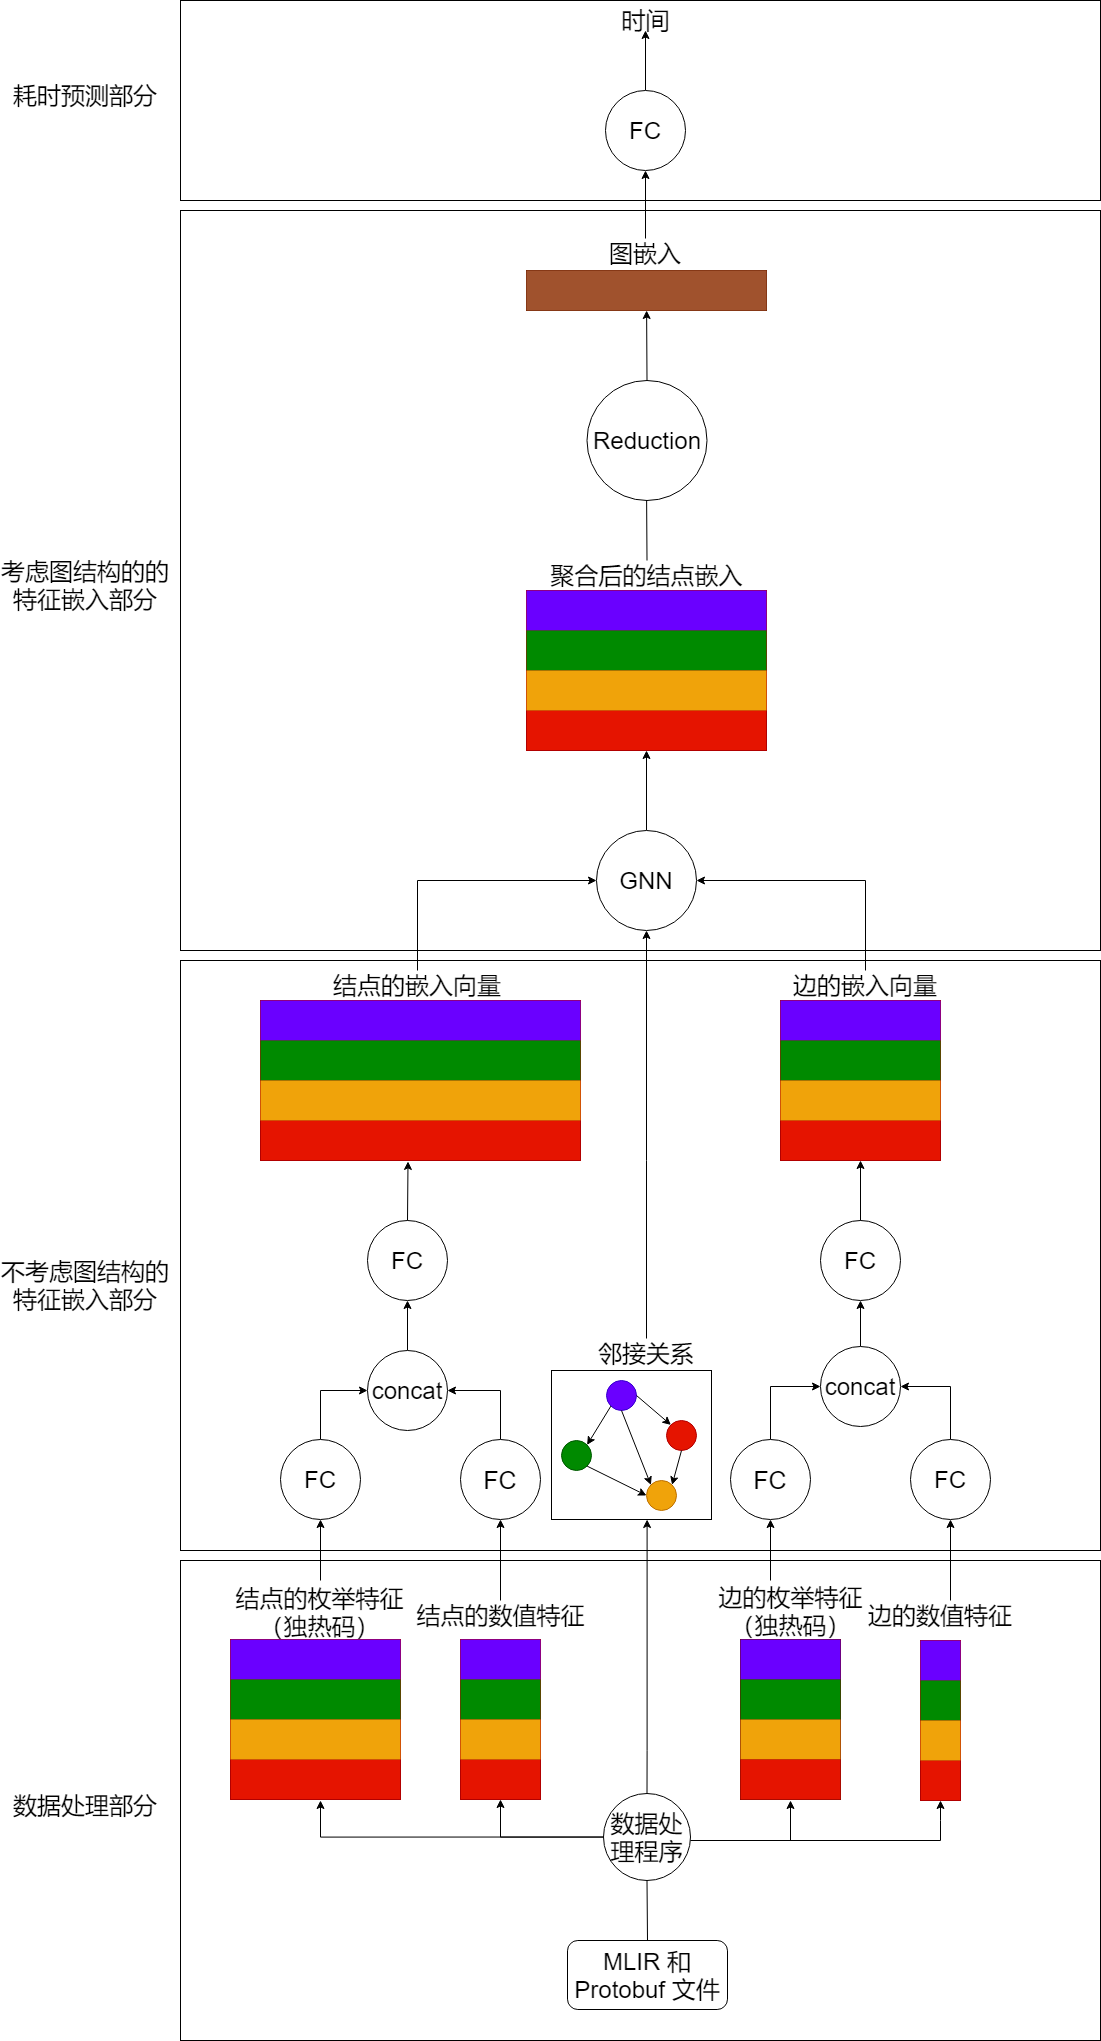
\includegraphics[width=0.85\textwidth,height=0.95\textheight]{figures/model.png}
    \caption{图神经网络耗时预测模型示意}
    \label{fig:graph8}
\end{figure}

以下为对上述模型的各个组成部分的说明。

\subsection{数据处理部分}
本文将 Y 编译器编译 ResNet-50 模型生成的若干个 MLIR 文件分别部署到不同 Protobuf 配置的硬件上(共计 126528 个组合),并测量了它们的实际运行时间作为数据集。

对于 MLIR 文件,本文使用正则表达式 \cite{regex} 提取计算图中结点的邻接关系以及结点和边的相关特征,按照提前统计的种类将枚举特征编码成独热码并将数值特征归一化后,以 pytorch \cite{NEURIPS2019_9015} 张量的形式保存到 DGL\cite{DGL} 的图结构中。

对于 Protobuf 文件,本文使用 Google 提供的处理 Protobuf 文件的工具 \cite{Google-pb} 提取其中的硬件特征,经过处理后拼接到结点对应的特征张量上。

\subsection{不考虑图结构的特征嵌入部分}
由于结点的不同特征对于该结点的执行时间会有不同权重的影响,而且同一种枚举特征的不同类型之间可能存在相似关系,故提取出的结点和边的特征需要采用可学习的方式嵌入到低维特征空间中。

本文采用分别将枚举特征和数值特征通过不同的全连接层后拼接起来,再通过同一个全连接层得到结点和边的嵌入向量,该嵌入向量作为图神经网络的输入。

\subsection{考虑图结构的特征嵌入部分}
由于边上的张量特征会影响其头结点和尾结点的执行时间,而不同结点的执行时间也可能会受到彼此特征的影响,故本文使用图神经网络聚集相邻结点和边的信息。

对于聚集得到的结点嵌入,本文将其归约以得到整个计算图的嵌入向量。谷歌\cite{Alearned}提出了多种归约方法,包括对结点嵌入进行逐元素运算、将结点嵌入
输入 LSTM \cite{LSTM1}, Transformer \cite{Transformer} 等模型从而生成图嵌入。
本文权衡训练时间和精度,最终选择将所有结点嵌入逐元素相加以得到计算图的嵌入。

\subsection{耗时预测部分}
本文将图嵌入向量的各个分量赋予可学习的权重,并相加得到耗时预测的时间。最后,本文计算预测时间与实际测量时间之间的损失函数,并通过反向传播更新模型的参数。

\section{损失函数与评价指标}

\subsection{损失函数}
损失函数在神经网络中用于刻画预测值与真实值的偏差,从而使用反向传播技术调整各层网络参数。
本文尝试的损失函数如下:
\subsubsection{MSE\cite{MSE}}
平均平方误差(mean squared error, MSE)是最常用的损失函数,其计算公式如下:
\begin{align}
    \mathbf{MSE} = \frac 1n \sum \limits_{i=1}^n (Y_i - \hat{Y}_i)^2
\end{align}
其中,$Y_i$ 为预测值,$\hat{Y}_i$ 为实际值,$n$ 为数据个数。

由于平方运算会放大误差,MSE 的缺点是容易受到较大或较小数据的影响。

\subsubsection{MAE\cite{MAE}}
平均绝对误差(mean absolute error, MAE)采用绝对值来代替平方运算,减少了极端数据对误差的影响:
\begin{align}
    \mathbf{MAE} = \frac 1n \sum \limits_{i=1}^n |Y_i - \hat{Y}_i|
\end{align}

由于本文所使用的数据集中存在规模较大和规模较小的计算图,故实际测量时间存在极端数据,所以本文最终使用 MAE 作为损失函数。

\subsection{评价指标}
评价指标用于衡量模型的泛化性,即模型在训练集之外的验证集和测试集上的预测效果。本文使用的评价指标如下:

\subsubsection{MAPE\cite{MAPE}}
平均绝对百分比误差(mean absolute percentage error, MAPE)是对 MAE 的改进:
\begin{align}
    \mathbf{MAPE} = \frac{100\%}{n}\sum\limits_{i=1}^n\left|\frac{Y_i-\hat{Y}_i}{\hat{Y}_i}\right|
\end{align}

由于平均绝对误差会受到数据整体数量级大小的影响,很难用于比较不同数据集之间的预测效果,故本文采用相对误差的平均值作为模型预测的评价指标之一。

\subsubsection{肯德尔秩相关系数\cite{Kendall}}
肯德尔秩相关系数(Kendall rank correlation coefficient)是用于衡量两个排序的相似程度的指标,其取值在 -1 和 1 之间,越接近 1 表示越相似。

若两个排序分别为 $x = (x_1,x_2, ..., x_n)$ 和 $y = (y_1,y_2, ..., y_n)$,则 $x$ 和 $y$ 之间的肯德尔秩相关系数计算如下:
\begin{align}
    \tau(x,y) = \frac{n_c-n_d}{\sqrt{(n_0-n_1)(n_0-n_2)}}
\end{align}
其中,$n_c$ 为所有满足 $i < j$ 的 $(x_i, x_j)$ 与 $(y_i,y_j)$ 中大小关系一致的 $(i,j)$ 对的个数,$n_d$ 为不一致的 $(i,j)$ 对的个数。
$n_0$ 为所有 $(i,j)$ 对的总数。$n_1$ 为 $x$ 排序中相同序号的对数,$n_2$ 为 $y$ 排序中相同序号的对数。

在本文所处理的问题中,为了进行编译优化配置的搜索,深度学习编译器只要能够比较不同硬件配置下计算图运行时间的相对大小即可,无需精确地估计每一种硬件配置对应的具体运行时间。

因此,本文也使用多个预测值和实际值之间的肯德尔秩相关系数作为衡量模型效果的指标。
在具体实验中,本文分别计算了同一个数据集内所有数据对应的肯德尔秩相关系数,以及每个 MLIR 在不同 Protobuf 配置\footnote{若某个 MLIR 仅对应一个 Protobuf 配置,则在计算时跳过该 MLIR。}下的预测时间和实际运行时间之间的肯德尔秩相关系数的平均值。
